\Large\textbf{Capitolo 4: \\DNA e cromosomi}

\section{Storia, scoperte ed esperimenti}
    \small
    L'informazione genetica di una cellula è contenuta all'interno dei cromosomi. Questi sono fatti di acidi nucleici e proteine le quali inizialmente si pensava fossero la base dell'informazione genetica.
    \subsection{Fredrick Griffith}
        Nel 1928, Griffith esegue un esperimento che certifica la trasformazione batterica. Prende due ceppi di Streptococcus pneumonae:
        \begin{itemize}
            \item ceppo S (smooth), patogeno per l'organismo topo
            \item ceppo R (rough), innocui per il topo
        \end{itemize}
        Si effettuano i seguenti esperimenti:
        \begin{enumerate}
            \item inoculo del ceppo S nel topo, il topo muore. Facendo una biopsia post mortem si riesce a risontrare lo stesso ceppo nell'organismo.
            \item inoculo del ceppo R nel topo, il topo non ne risente.
            \item inoculo del ceppo S inattivato al calore nel topo, il topo non ne risente.
            \item inoculo del ceppo S inattivato al calore insieme al ceppo R nel topo, il topo sviluppa la malattia e muore. Facendo una biopsia si riscontra il ceppo S.
        \end{enumerate}
        Si deduce che avviene una cerca comunicazione tra i batteri per lo scambio di informazioni, si parla quindi di \textit{trasformazione batterica}.
        
    \subsection{Avery, MacLeod e McCarty}
    Nel 1944, questi scienziati condussero esperimenti sul ceppo patogeno S di cui si è parlato nell'esperimento precedente. In particolare il ceppo S viene esposto a tre enzimi:
    \begin{enumerate}
        \item DNAasi
        \item RNAasi
        \item Proteinasi
    \end{enumerate}
    Si osserva che solo nel primo caso il ceppo non è più in grado di eseguire la trasformazione batterica di cui si parlava nell'esperimento precedente. Di conseguenza il DNA degradato era responsabile per il trasferimento dell'informazione genetica.
    
    \subsection{Hershey e Chase}
    Nel 1952, Hershey e Chase usarono un batteriofago T2 contro E. Coli. Si era a conoscenza che il fago contenesse le informazione genetiche per produrre copie di se stesso e si sapeva che il virus fosse composto solo di DNA e proteine. \\
    \begin{enumerate}
        \item Si marcarono le proteine con l'isotopo S35 e il DNA con P32. 
        \item E. Coli ospita i fagi e ne avviene la replicazione
        \item Il tutto viene centrifugato per ottenere l'isolamento delle molecole pesanti.
    \end{enumerate}
    Il battere infettato contiene P32, di conseguenza è il DNA a veicolare l'informazione genetica.
    
    \subsection{Watson, Crick e Franklin}
    Nel 1953, questi tre scienziati cercarono di comprendere la struttura tridimensionale della molecola del DNA. Si scoprì che è composta dalle quattro basi azotate legate tra loro attraverso un numero differente di legami H (tre per la coppia CG e due per AT). 
    Grazie alla cristallografia a raggi X, si dedusse la conformazione a doppia elica del DNA associate in maniera antiparallela.\\
    Si giunse alla conclusione che ogni cellula racchiudeva il meccanismo per la sua duplicazione, trasferendo alla cellula figlia la stessa informazione genetica.
    
\section{Struttura}
    \small
    La cellula eucariotica è diploide (ad esclusione dei gameti), quelle umane comprendono circa 3.2 miliadri di pb, divisi in 22 coppie di cromosomi più una sessuale.\\
    I geni sono le sequenze del DNA deputate alla produzione di proteine, nell'uomo le sequenze codificanti sono meno dell'1\%.
    Il DNA intergenico ha tuttora funzioni ignote, tuttavia certamente non codificanti. \\
    Per traslocazione si intende lo spostamento di specifiche porzioni del genoma in porzioni differenti del DNA, causando possibilmente un fenotipo patologico. Questo tipo di eventi avviene spesso nelle cellule tumorali.
    
    \subsection{Fasi del ciclo cellulare}
        Le fasi del ciclo di vita della cellula si possono dividere in:
        \begin{itemize}
            \item Interfase, composta da fase G0 (fase di vita cellulare esonerata dal ciclo replicativo), G1 (periodo durante il quale si costituiscono nuovi componenti per fare fronte alle fasi successive), S (\textit{sintesi}, viene sintetizzato nuovo DNA) e G2 (nuovo periodo in cui accrescono le quantità di molecole necessarie).
            \item Fase M, ovvero la mitosi (divisa in profase, prometafase, metafase, anafase e telofase). Durante la mitosi avviene la compattazione del materiale genetico in cromosomi e la segregazione ai poli.
        \end{itemize}
    
     \begin{figure}[h]
            \centering
            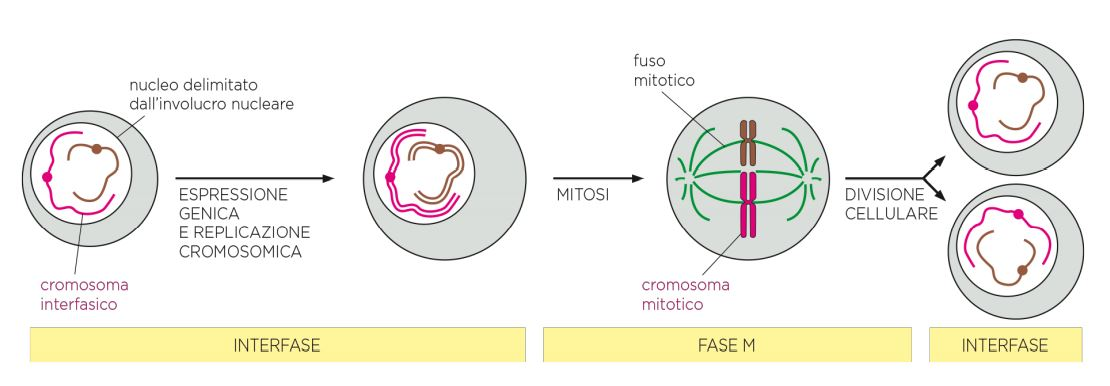
\includegraphics[width=1\textwidth]{images/mitosiBreve.JPG}
            \caption{\small fasi del ciclo cellulare in breve}
            \label{fig:mesh1}
        \end{figure}
    
    \subsection{Cromosomi eucariotici}
        I cromosomi sono composti da due cromatidi fratelli, un centromero, molteplici origini di replicazione (ORI), i telomeri alle estremità.\\
        Durante la fase M, ORI viene localmente "aperto" e si procede alla sintesi di un nuovo filamento sullo stampo dei due disponibili. I due cromatidi sono tenuti assieme dal centromero che consentono interazioni con elementi citoschelettrici.
        I telomeri sono sequenze nucleotidiche alle estremità del filamento che consentono la replicazione di queste.\\
        Durante la fase I, il DNA è molto più svolto all'interno del nucleo formando la cromatina. Si nota comunque che cromosomi diversi sono confinati in aree specifiche della cromatina.\\
        Il DNA può assumere due gradi di avvolgimento:
        \begin{itemize}
            \item regioni eterocromatiniche, zone che contengono geni non esprimibili a causa dell'elevata compattezza
            \item regioni eucromatiniche, sono la maggioranza e possono contenere geni esprimibili.
        \end{itemize}
        
        \subsubsection{Riavvolgimenti e compattazione}
            Per \textit{nucleosoma} si intende il DNA avvolto su dischi proteici, ovvero gli \textit{istoni}, per la formazione di una struttura a \textit{collana di perle}. Attorno all'istone si arrotolano 1.7 giri di DNA. 
            Tra una proteina e l'altra di identifica il DNA di connessione. Questa struttura può essere disassemblata da enzimi che conducono attività nucleasica.\\
            
            \textbf{Istoni}\\
                Il disco proteico è composto da otto istoni (subunità), in particolare di quattro polipeptidi, ognuno presente in due copie: H2A, H2B, H3 e H4.\\
                Sono molto basiche (per legare il DNA carico negativamente), l'N-terminale protrude all'esterno del disco per ogni istone, sono proteine estremamente conservate tra speci diverse. Il DNA avvolto attorno ai dischi risulta 3 volte più corto.\\
                L'istone H1 non fa parte del core dell'ottamero, ma si associa a nucleosomi differenti e trasforma la struttura in fibra cromatinica. Non è ancora conosciuto il procedimento attraverso il quale il DNA si ripieghi formando anse.
                Nel caso della porzione di DNA su cui si andrà a formare il cinetocore si ha una differenza locale nella struttura istonica (CEMP-A al posto di H3, dalla quale dipende la formazione delle altre proteine del cinetocore).
                
            \begin{figure}[h]
                \centering
                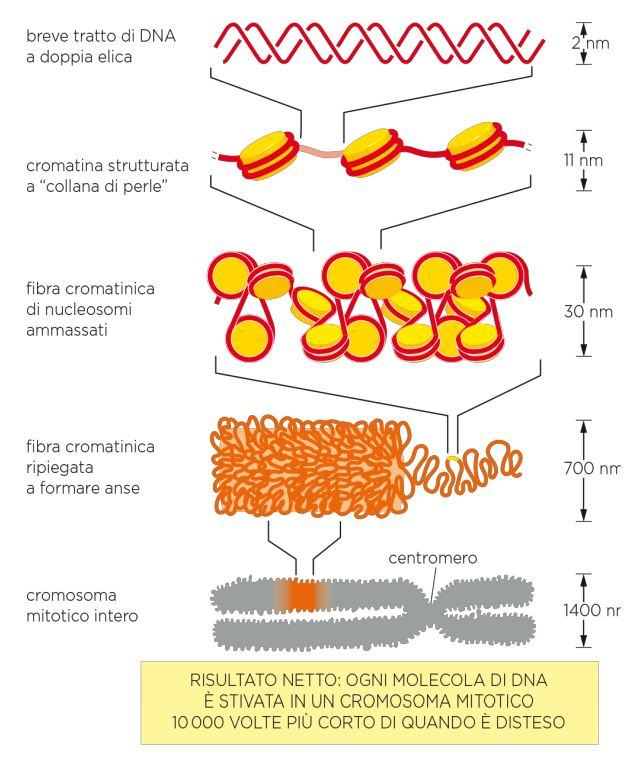
\includegraphics[width=0.75\textwidth]{images/compattazioneDNA.JPG}
                \caption{\small schema degli stadi della compattazione del DNA in cromosomi}
                \label{fig:mesh1}
            \end{figure}
        
        \subsubsection{Svolgimenti e decompattazione}
            Lo svolgimento del materiale genetico richiede energia ed è dunque sfavorito. Sono dunque necessari dei complessi per la decondensazione della cromatina. Ogni N-terminale degli istoni può subire delle modifiche chimiche post traduzionali che fungono da segnale: determinano la struttura 3D e hanno significati diversi, ad esempio possono indicare lo spegnimento del gene o il suo aumento di espressione.\\
            L'accessibilità della sequenza nucleotidica ne determina l'espressione:
            \begin{enumerate}
                \item eucromarina: è la porzione più abbondante e rappresenta contenuto accessibile ed esprimibile
                \item eterocromatina: è una porzione non accessibile e non esprimibile, ne fanno parte telomeri e centromero.
                \item porzioni intermedie
            \end{enumerate}
            L'accessibilità à determinata dalle modifiche istoniche della cromatina: una modifica dell'istone può propagarsi "automaticamente" fino a una determinata sequenza isolante che funge da barriera.\\
            Nel caso di un individuo di sesso femminile, vengono utilizzate le informazioni presenti solamente su uno dei due cromosomi sessuali, per questo uno dei due viene "spento" effettuando per l'appunto modifiche post traduzionali dell'istone. In alcuni casi (come quello del gatto calico) vengono silenziate zone solo localmente. Questo avviene in fasi precoci dell'embriogenesi.
        
\section{Duplicazione}
    Ogni filamento di DNA viene usato come stampo per la sintesi di una nuova molecola di DNA completa. Il processo avviene in maniera semiconservativa. I legami H tra le basi azotate conferiscono grande stabilità alla molecola, per denaturare la struttura occorre aumentare la temperatura superando i 95° C. \\
    La temperatura di melting tuttavia dipende dalla percentuale di basi azotate presenti sul filamento: infatti se sono presenti più G o C, la temperatura di denaturazione sarà più alta perché sono legate attraverso tre interazioni H al posto di due (quelle tra A e T). 
    In particolare si assume una regola spannometrica per cui per ogni C o G si aumenta la temperatura di 4° e per ogni A e T si aumenta di 2°.\\
    Tuttavia nella fase di replicazione, il DNA deve essere localmente denaturato per consentire l'appaiamento delle basi, in questo caso la temperatura sarà stabile a 37°C e la denaturazione non sarà mediata dalla temperatura.
    L'inizio della denaturazione del DNA per la replicazione avviene in una zona che comprende A e T per facilitare il processo.\\
    L'origine della replicazione nel genoma batterico è identificata da un'unica ORI, perché il cromosoma. In più non sono presenti istoni.
    Per le cellule eucariotiche, e in particolare quelle umane, esistono più di 10.000 ORI differenti, più di una per ogni cromosoma.
    
    \subsection{Teorie di replicazione}
        Le teorie sulla replicazione del DNA si dividevano in tre categorie:
        \begin{enumerate}
            \item conservativa: il nuovo filamento di DNA sintetizzato non eredita fisicamente nessuna porzione del DNA padre ma è tutto prodotto ex novo.
            \item semi-conservativa: un filamento di ogni molecola di DNA deriva dal padre.
            \item dispersiva: ogni filamento del padre è segmentato e ricucito tra due figli, ogni filamento contiene delle porzioni randomiche derivanti dal padre.
        \end{enumerate}
        \subsubsection{Meselson e Stahl}
            Nel 1958, questi due scienziati provarono la semiconservatività del processo di duplicazione del DNA. In particolare prepararono due colture batteriche marcate rispettivamente con isotopi di N15 e N14. La densità del primo risulterà maggiore di quella del secondo.\\
            Queste due colture vengono messe in contatto e si lasciato incubare nuovamente. Successivamente, centrifugando il campione ottenuto si osserva che i batteri formavano uno strato omogeneo: questo condusse ad un esclusione della teoria conservativa perché se quello fosse stato il caso sarebbero state visibili due bande distinte.\\
            Sottoponendo poi il DNA delle colture ad una denaturazione, si è potuto notare che si venivano a formare due fasce ben definite, prova del fatto che la duplicazione del DNA avviene in maniera semi-conservativa (se così non fosse stato, si sarebbe riscontrata una fascia uniforme).
        
        \subsection{Neosintesi}
            Il processo di neosintesi comincia con la formazione di una forcella replicativa (locale denaturazione del DNA) e la sintesi avviene su entrambi i filamenti esposti, quindi bidirezionale. \\
            L'enzima che catalizza la sintesi è la DNA Polimerari (DNA-P) che aggiunge nuovi nucleotidi in direzione 5' - 3'. La sintesi quindi avviene solo sull'estremità 3'.\\
            Il filamento stampo determina la sequenza nucleotidica, le basi vengono legate tra loro tramite un legame fosfodiesterico, rilasciando una molecola di acqua (consensazione).\\
            Muovendosi, la forcella replicativa denatura i filamenti di cui uno risulta leggibile da 5' - 3' mentre uno da 3' - 5'.
            \subsubsection{Leading strand}
                Il filamento che viene letto in direzione 5' - 3' è detto \textit{leading strand} e la sua sintesi avviene in modo continuativo ad opera della DNA-P.
            
            \subsubsection{Lagging strand}
                Il filamento disponibile in direzione 3' - 5' non può essere sintetizzato in maniera diretta dalla DNA-P perchè essa può procedere solo aggiungendo nucleotidi all'estremità 3'. Per questo la DNA-P sintetizza nuovo DNA in frammenti 5' - 3' (Okazaki fragments) che verranno poi "ricuciti" successivamente.
            
            \begin{figure}[h]
                \centering
                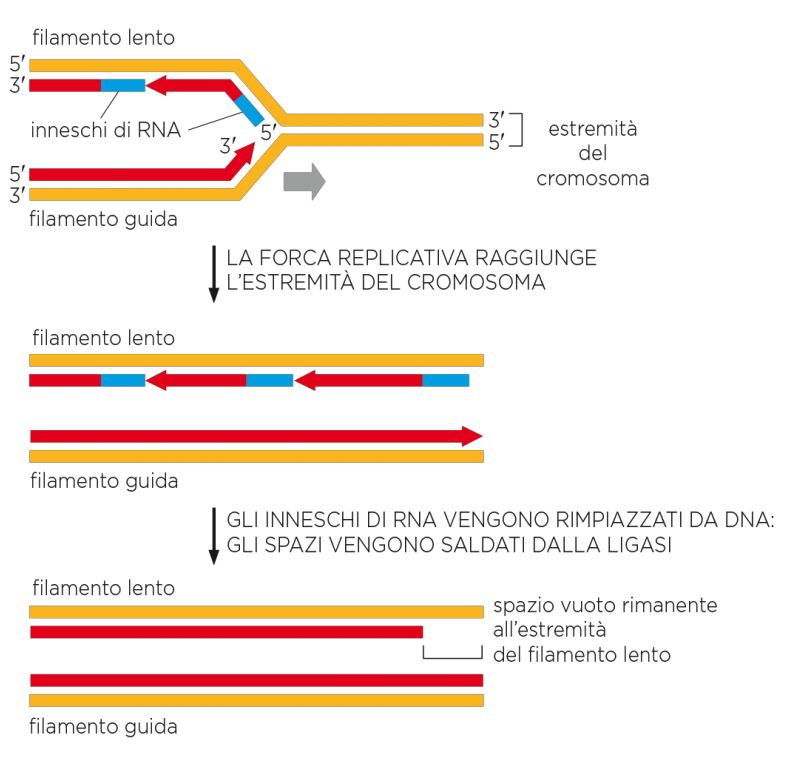
\includegraphics[width=0.75\textwidth]{images/forcellareplicativa.JPG}
                \caption{\small forcella replicativa, frammenti di Okazaki, leading strand e lagging stand}
                \label{fig:mesh1}
            \end{figure}
        
        \subsection{DNA-polimerasi}
            La DNA-P è formata da due domini funzionali:
            \begin{itemize}
                \item un dominio P: consiste nel sito catalitico per la polimerizzazione
                \item un dominio E: che funge da sito catalitico per l'autocorrezione
            \end{itemize}
            La direzione per la polimerizzazione è unica (verso 3') e per sintetizzare il reato del filamento anche partendo da uno già esistente ossia una sequenza \textit{primer}.  \\
            Un primer è uno stratch nucleotidico complementare in ORI?? che è necessario per iniziare l'attività di DNA-P. Consiste in un frammento di RNA di circa 10 pb sintetizzato dalla primasi.\\
            Per il lagging strand ci sono delle sequenze primer per ogni frammento di Okazaki. Nel momento in cui DNA-P raggiunge un primer dopo aver sintetizzato il frammento, interviene un enzima che degrada il primer e una specifica DNA-P (*) prosegue utilizzando le basi con desossiribosio corrette: questa è meno processiva di DNA-P menzionata fino ad ora per limitare i danni.
            Successivamente interviene la DNA ligasi che forma il legame tra i due frammenti di Okazaki.
            \subsubsection{Errori di sintesi}
                Gli errori di posizionamento di un nucleotide sono molto rari: circa 1 su 10.000.000 questo perchè i legami corretti sono favoriti energicamente.\\
                catalisi qualcosa?\\
                La DNA-P eucariotica avvolge un'attività di \textit{proof reading}, per cui viene controllato l'appaiamento corretto della base appena inserita, nel caso in cui si percepisca il difetto, viene liberato il nucleotide e DNA-P riprende.
                
        \subsection{Step della sintesi}
            \begin{enumerate}
                \item \textbf{attività dell'elicasi}\\
                L'elicasi idrolizza ATP per catalizzare la denaturazione del filamento. La DNA-P lavora subito dopo la denaturazione così da evitare che le basi si riassocino (per il leading strand). Il lagging strand invece rimane singolo finchè non interviene la primasi.\\
                Esistono delle \textit{single strand DNA binding proteins} che evitano che il filamento di DNA si ripieghi su se stesso.
                \item \textbf{clamp}\\
                La DNA-P si associa al filamento e viene mantenuta tale da un trimero chiamato \textit{ sliding clamp}, negli eucarioti \textit{PCNA} ovvero \textit{Proliferating cell nuclear antigen}.
                \item \textbf{topoisomerasi}\\
                Vi è la formazione di una tensione sul DNA non denaturato che viene risolta dalla topoisomerasi che opera dei piccoli "tagli" su un filamento in modo da eliminare i superavvolgimenti (e successivamente interviene la ligasi per riallacciare la sequenza).
                \item \textbf{telomeri}\\
                Non è possibile secondo questo procedimento procedere alla sintesi dell'inizio della sequenza del lagging strand in 5'. Per evitare l'accorciamento del DNA a scapito di sequenze utili, sono presenti le sequenze telomeriche all'estremità 3' del filamento. Sono delle porzioni di DNA con delle caratteristiche specifiche:
                \begin{itemize}
                    \item sono delle sequenze segnale che invocano l'intervento di cromatina dedicata per la protezione delle estremità ??? eterocromatina
                    \item forniscono meccanismo per la sintesi delle estremità tramite una ribonucleoproteina che aggiunge sequenze su un filamento stampo consentendo l'appaiamento della fine del DNA.
                \end{itemize}
            \end{enumerate}
            \begin{figure}[h]
                \centering
                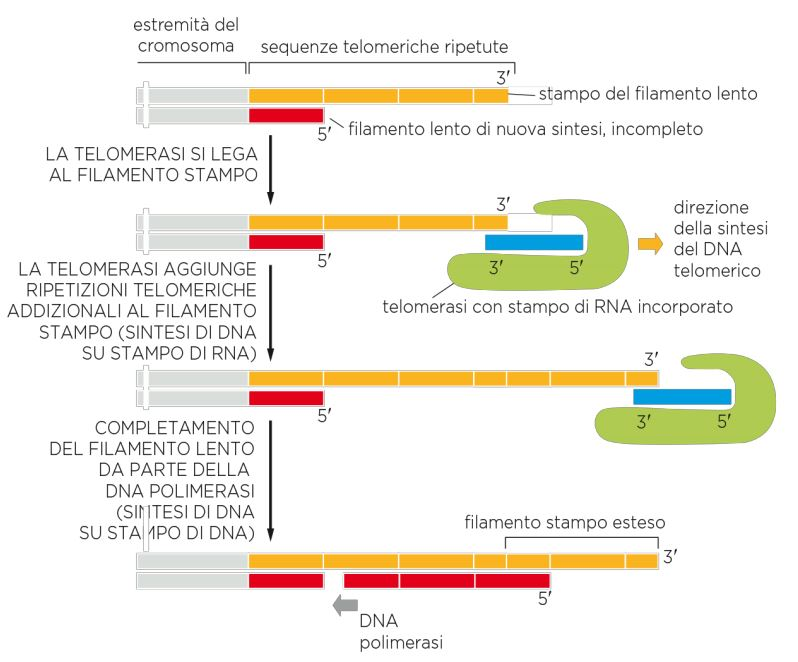
\includegraphics[width=0.75\textwidth]{images/telomero.JPG}
                \caption{\small funzionamento della sequenza telomerica}
                \label{fig:mesh1}
            \end{figure}
            
            \subsubsection{telomeri e senescenza}
                Nelle celllule somatiche gli enzimi per la telomerasi non sono espresse e la sequenza telomerica si accorcia ad ogni ciclo di replicazione. 
                Al contrario nelle cellule uovo e negli spermatozoi al sequenza telomerica raggiunge la sua lunghezza massima.\\
                Per senescenza si intende il processo degradativo della cellula a causa della perdita dei porzioni telomeriche.\\
                
                \textbf{Esperimento di Hayflick}\\
                Nel 1962, Hayflick condusse un esperimento su cellule epiteliali. Se ne favorisce la proliferazione e si nota che questo processo non viene sostenuto per una quantità temporale indeterminata:
                si evidenzia una fase di crisi dopo circa 50 duplicazioni per poi fare fronte al decadimento effettivo della coltura. Le cellule restano in vita ma non proliferano.\\
                Nelle cellule di un neonato questo processo avviene dopo a confronto di cellule di un anziano. Si associa alla senescenza l'esaurimento delle sequenze telomeriche.
\section{Mutazioni}
    Le mutazioni a livello di sequenza nucleotidica possono causare gravi patologie o essere incompatibili con la vita.
    \subsection{Processi spontanei}
        \subsubsection{Depurinazione}
            Per depurinazione si intende la perdita di una purina per idrolisi. Avviene perchè la DNA-P perde una base nel processo di sintesi.
        \subsubsection{Deamminazione della citosina}
            La citosina perde un gruppo amminico e diventa uracile. Nelle replicazioni successive verrà inserita una adenina al posto di una guanina.
    
    \subsection{Altri processi}
        \subsubsection{Dimeri di timina}
            La formazione di dimeri di timina non è un processo spontaneo ma aumenta all'aumentare delle radiazioni. Si effettua un legame chimico tra due timine sullo stesso filamento, quando la DNA-P cerca di sintetizazre il filamento non riesce ad interpretare la base da associare.
        \subsection{Radiazioni ionizzanti}
            Vengono introdotti ioni nella struttura chimica del DNA rompendo la struttura stessa.
            I telomeri vengono protetti da cappucci proteici.
            Le terminazioni del DNA possono essere ricucite da una ligasi secondo due alternative:
            \begin{itemize}
                \item \textbf{non omologus ends join}: la ligasi salda qualunque estremità piatta, senza cappucci proteici o telomeri. Questo tipo di saldatura è prona ad errori e può succedere in inserimento o una delezione di una base.
                \item \textbf{omologus ends join}: avviene solamente qualora il DNA sia già stato replicato e il duplex danneggiato è prossimo a quello omologo. La cellula cerca la sequenza non danneggiata per aggiustare il filamento danneggiato.
            \end{itemize} 
            Per esempio l'anemia falciforme è dovuta ala mutazione di un unico nucleotide, la stessa mutazione ha riscontrato una certa importanza nella difesa della malaria (nelle zone del mondo in cui la malaria è più diffusa è anche più diffuso questo tipo di anemia).\\
        
     \subsection{Metodi di riparazione}
        \subsubsection{Nucleotide excision repair}
            Viene scisso il nucleotide sbagliato e viene sostituito da DNA-P(*), successivamente interviene la ligasi.
        \subsubsection{Mismatch repair}
            Viene tolta la base sabagliata e viene corretta, non è scontato sapere quale delle due basi sui due filamenti sia quella corretta.

\pagebreak